\begin{itemize}
  \item Una prueba de ejecucion es la siguiente.\\ 
  Observando la tabla de excel generada podemos observar que contamos con 10 documentos, de los cuales ya tenemos su matris binaria para identificar que palabra esta en cada documento, y con ello poder realizar la busqueda de palabras clave en cada documento.
  \begin{figure}[ht]
    \centering
    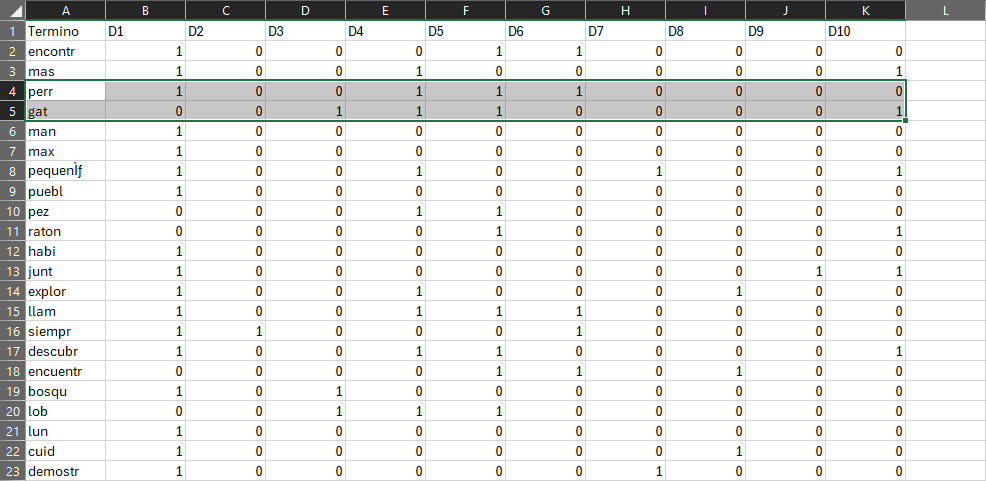
\includegraphics[width=0.8\textwidth]{src/img/resultado/1.png}
    \caption{Resultado}
  \end{figure}
  \item Para este caso nos vamos a centrar en las palabras clave "cachorro" y "angel" para poder determinar el funcionamiento de nuestra aplicacion de busqueda por metodo booleano.
  \begin{figure}[ht]
    \centering
    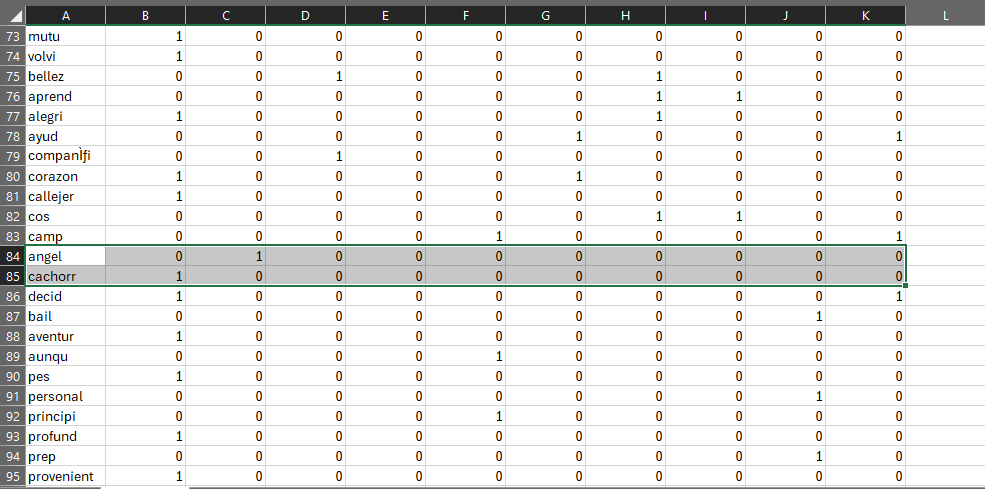
\includegraphics[width=0.8\textwidth]{src/img/resultado/2.png}
    \caption{Resultado}
  \end{figure}
  \newpage
  \item como podemos observar en la aplicacion tenemos un apartado donde podemos ingresar la exprecion booleana que deseamos buscar.
  \begin{figure}[ht]
    \centering
    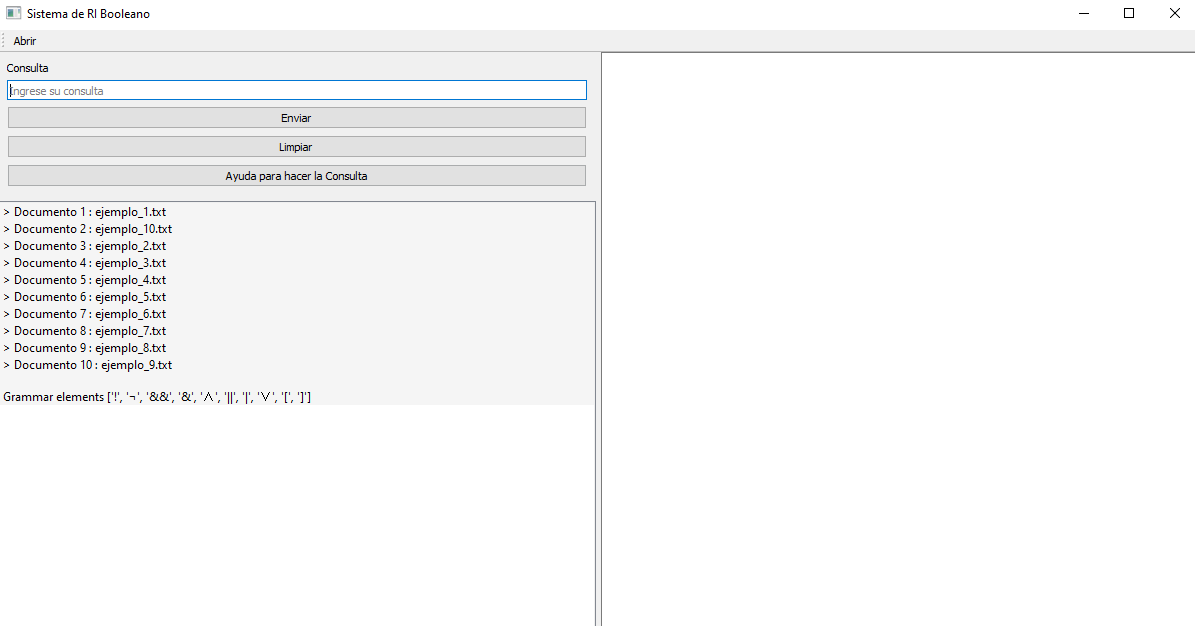
\includegraphics[width=0.8\textwidth]{src/img/resultado/3.png}
    \caption{Resultado}
  \end{figure}
  \item En este caso vamos a buscar la palabra "cachorro" o "angel", para ello ingresamos la exprecion "cachorro | angel" y damos click en el boton de buscar, con ello nos mostrara los documentos que contienen la palabra "cachorro" o "angel", en este caso solo el documento 1 y 2 contienen la palabra "cachorro" o "angel".
  \begin{figure}[ht]
    \centering
    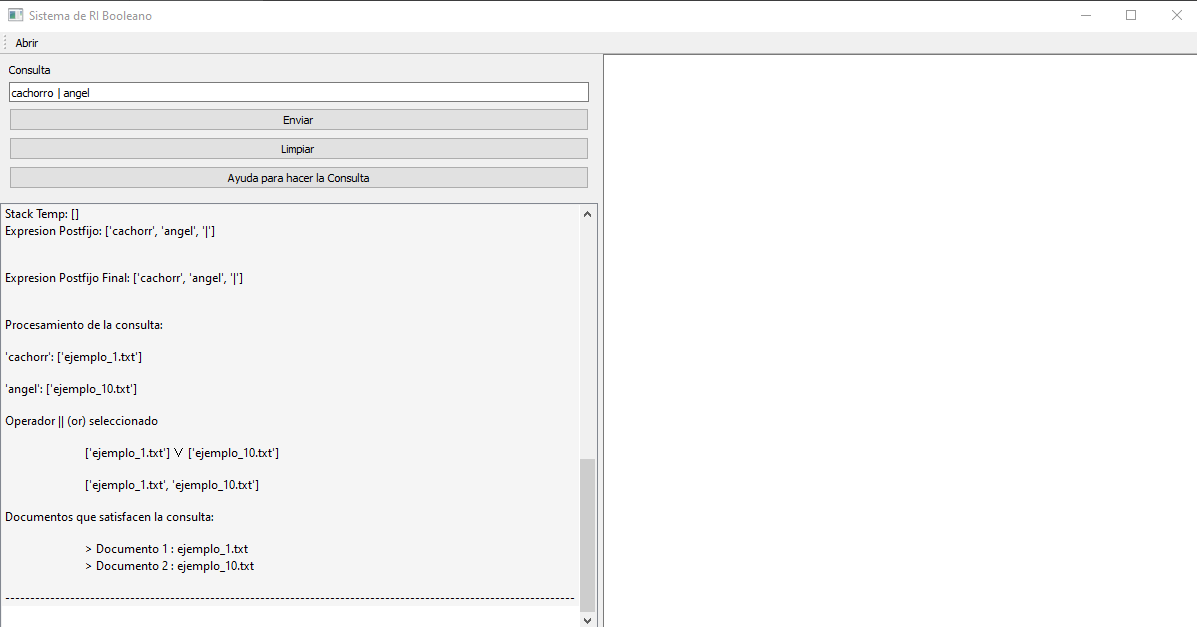
\includegraphics[width=0.8\textwidth]{src/img/resultado/4.png}
    \caption{Resultado}
  \end{figure}
  \newpage
  \item Ahora bien si deseamos buscar la palabra "cachorro" y "angel" en los documentos, ingresamos la exprecion "cachorro \& angel" y damos click en el boton de buscar, con ello nos mostrara los documentos que contienen la palabra "cachorro" y "angel", en este caso no hay documento que cumpla con la condicion.
  \begin{figure}[ht]
    \centering
    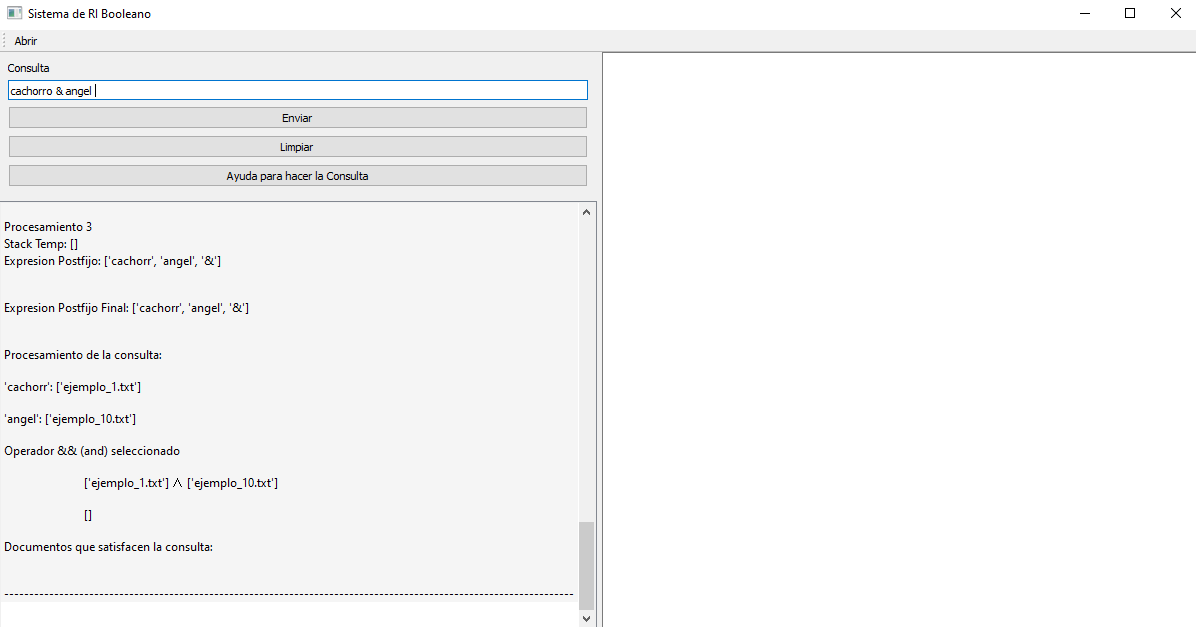
\includegraphics[width=0.8\textwidth]{src/img/resultado/5.png}
    \caption{Resultado}
  \end{figure}
  \item Pero que pasa si a toda la exprecion le agregamos un "not", en este caso vamos a buscar la palabra "cachorro" y "angel" en los documentos, ingresamos la exprecion "\! ( cachorro \& angel )" y damos click en el boton de buscar, con ello nos mostrara los documentos que no contienen la palabra "cachorro" y "angel", en este caso son todos los documentos que no contienen la palabra "cachorro" y "angel" en el mismo documento.\\
  \begin{figure}[ht]
    \centering
    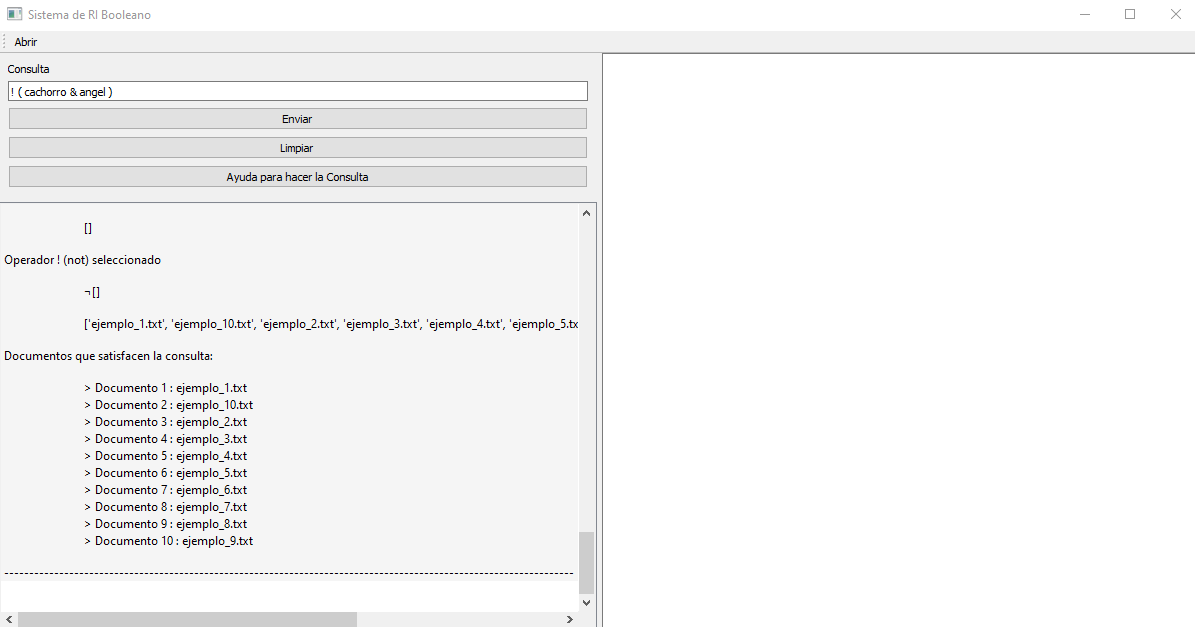
\includegraphics[width=0.8\textwidth]{src/img/resultado/6.png}
    \caption{Resultado}
  \end{figure}
\end{itemize}
